\chapter{Plotting with Matplotlib}
\label{ch:matplotlib} 

\begin{flushright}
	\parbox{8cm}
		{
		\begin{flushright}
		\rule{8cm}{0.5pt}\\
		\vspace*{5mm}
		\sffamily \
		Reading:\\
		\href{http://matplotlib.sourceforge.net/}{Matplotlib Web Site}
		
		\vspace*{5mm}
		\rule{8cm}{0.5pt}
		\end{flushright}
		}
\end{flushright}


\section{Plotting a function}\label{sec:functionPlot}
Sometimes you need a quick plot of a function. In Listing~\ref{plot}, I have a simple example of this. Let's assume that you want to plot a more complicated function; say 
\begin{equation} y = \sin(t^2) \label{eq:sineSquared}\end{equation}
\\
\rule{\textwidth}{1pt}
\begin{exercise}\label{exer:plotFuncSineSquared}
Go ahead and write a python script called \verb!plotFunction.py! that displays this Equation~\ref{eq:sineSquared}. Is your plot reasonable? Why or why not? If it's not reasonable, fix the code so that it gives a reasonable plot!
\end{exercise}
\rule{\textwidth}{1pt}

\section{Plotting data from a text file}
Imagine you're in a lab and you've recorded some (x,y) data points in your laboratory notebook and you want to make a plot of this data. Because you are a scientist, you have uncertainties associated with each of these values and you want your plot to include error bars. 
You can of course, use some scientific plotting program to do this, or you can use python. Suppose you have entered data into a text file and you have the following data (Table~\ref{tab:sampleData})
\begin{table}
\caption{Imaginary data from your lab notebook; assume that the time uncertainties are all equal to 0.2 s.}\label{tab:sampleData}
\vspace*{3mm}
\begin{tabular}{crr}
\toprule
time (s)	& Temp (C)	& $\Delta$T (C)\\
\midrule
0.2		& 8.24	 & 0.9\\
0.4		& 13.76	 & 0.8\\
0.6		& 17.47	 & 0.7\\
0.8		& 19.95	 & 0.6\\
1.0		& 21.62	 & 0.5\\
1.2		& 22.73	 & 0.4\\
1.4		& 23.48	 & 0.3\\
1.6		& 23.98	 & 0.2\\
1.8		& 24.32	 & 0.1\\
2.0		& 24.54	 & 0.1\\
\bottomrule
\vspace*{4mm}
\end{tabular}
\end{table}

\begin{exercise}
	Using the ``data'' in Table~\ref{tab:sampleData}, use numpy and matplotlib to plot the data, complete with errorbars and axes lables. Your result should look like Figure~\ref{fig:sampleDataPlot}. Your report should include a duplicate of the Table~\ref{tab:sampleData}, your python code, and the plot created by matplotlib.
\end{exercise}


\begin{figure}[htb]
  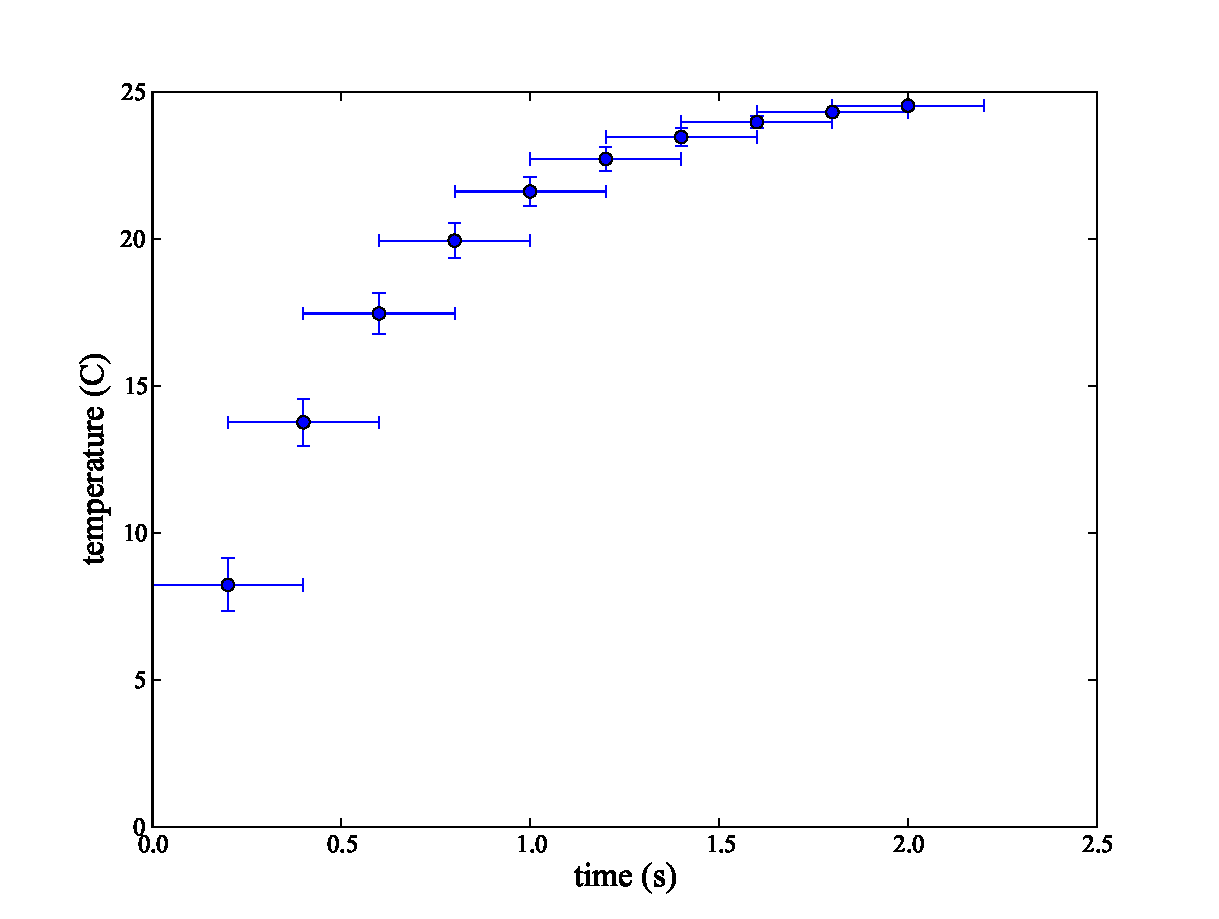
\includegraphics[width=.85\linewidth]{Figures/SimplePlots/dataPlot.pdf}%
  \caption{A plot of the data shown in Table~\ref{tab:sampleData}.}
  \label{fig:sampleDataPlot}%
\end{figure}

